% Options for packages loaded elsewhere
\PassOptionsToPackage{unicode}{hyperref}
\PassOptionsToPackage{hyphens}{url}
%
\documentclass[
]{article}
\usepackage{lmodern}
\usepackage{amssymb,amsmath}
\usepackage{ifxetex,ifluatex}
\ifnum 0\ifxetex 1\fi\ifluatex 1\fi=0 % if pdftex
  \usepackage[T1]{fontenc}
  \usepackage[utf8]{inputenc}
  \usepackage{textcomp} % provide euro and other symbols
\else % if luatex or xetex
  \usepackage{unicode-math}
  \defaultfontfeatures{Scale=MatchLowercase}
  \defaultfontfeatures[\rmfamily]{Ligatures=TeX,Scale=1}
\fi
% Use upquote if available, for straight quotes in verbatim environments
\IfFileExists{upquote.sty}{\usepackage{upquote}}{}
\IfFileExists{microtype.sty}{% use microtype if available
  \usepackage[]{microtype}
  \UseMicrotypeSet[protrusion]{basicmath} % disable protrusion for tt fonts
}{}
\makeatletter
\@ifundefined{KOMAClassName}{% if non-KOMA class
  \IfFileExists{parskip.sty}{%
    \usepackage{parskip}
  }{% else
    \setlength{\parindent}{0pt}
    \setlength{\parskip}{6pt plus 2pt minus 1pt}}
}{% if KOMA class
  \KOMAoptions{parskip=half}}
\makeatother
\usepackage{xcolor}
\IfFileExists{xurl.sty}{\usepackage{xurl}}{} % add URL line breaks if available
\IfFileExists{bookmark.sty}{\usepackage{bookmark}}{\usepackage{hyperref}}
\hypersetup{
  pdftitle={the motivating use-case for simeta::},
  hidelinks,
  pdfcreator={LaTeX via pandoc}}
\urlstyle{same} % disable monospaced font for URLs
\usepackage[margin=1in]{geometry}
\usepackage{graphicx}
\makeatletter
\def\maxwidth{\ifdim\Gin@nat@width>\linewidth\linewidth\else\Gin@nat@width\fi}
\def\maxheight{\ifdim\Gin@nat@height>\textheight\textheight\else\Gin@nat@height\fi}
\makeatother
% Scale images if necessary, so that they will not overflow the page
% margins by default, and it is still possible to overwrite the defaults
% using explicit options in \includegraphics[width, height, ...]{}
\setkeys{Gin}{width=\maxwidth,height=\maxheight,keepaspectratio}
% Set default figure placement to htbp
\makeatletter
\def\fps@figure{htbp}
\makeatother
\setlength{\emergencystretch}{3em} % prevent overfull lines
\providecommand{\tightlist}{%
  \setlength{\itemsep}{0pt}\setlength{\parskip}{0pt}}
\setcounter{secnumdepth}{5}

\title{the motivating use-case for simeta::}
\author{}
\date{\vspace{-2.5em}}

\begin{document}
\maketitle

{
\setcounter{tocdepth}{2}
\tableofcontents
}
\hypertarget{important-message-for-future-charles}{%
\subsubsection{Important message for future
Charles:}\label{important-message-for-future-charles}}

\textbf{Remember, writing this provides a fun and aesthestic way of
debugging this algorithm. Focus on writing a cohesive document, and the
debugging will be enjoyable. It's a cognitive bait and switch; and it
works. Make the document \emph{pretty}, and you not be able to help
ensuring the science is correct, because you hate doing a sloppy job at
anything. Answer the question, with clarity and aesthetics; the
motivation for correct science will follow.}

\hypertarget{preamble}{%
\subsection{preamble}\label{preamble}}

\begin{verbatim}
library(simeta)
library(varameta)

# other packages used in this vignette
library(tidyverse)
library(skimr)

# otherwise i'll forget
conflicted::conflict_prefer("filter", winner = "dplyr")

# for reproducibility
set.seed(39)
\end{verbatim}

\hypertarget{objective-of-the-simeta-package}{%
\section{\texorpdfstring{Objective of the \texttt{simeta::}
package}{Objective of the simeta:: package}}\label{objective-of-the-simeta-package}}

The \texttt{simeta::} package aims to provide coverage probability
simulation results for estimators derived, as is common in
meta-analyses, from summary statistics for the variance of the sample
median.

Different simulation-level parameters of interest can be specified so
that simulated data mimics different meta-analytic conditions:

\begin{itemize}
\tightlist
\item
  Different numbers of \(K\) studies.
\item
  Different values of \(\tau^2\), the variation between the studies.
\item
  Different distributions.
\item
  Different distributions of expected sample sizes.
\item
  Different proportions of control and intervention group.
\end{itemize}

The components of the algorithm have been produced in a
compartmentalised way, with the objective of exploring the extendability
of this package to estimators for the variance of the sample mean, but
also for estimators for the mean or median, themselves.

In this vignette, we restrict ourselves to the original use-case of the
package, testing estimators for the variance of the sample median.

\hypertarget{using-simeta-to-assess-an-estimator-for-the-sample-median}{%
\section{\texorpdfstring{Using \texttt{simeta::} to assess an estimator
for the sample
median}{Using simeta:: to assess an estimator for the sample median}}\label{using-simeta-to-assess-an-estimator-for-the-sample-median}}

Taking a case study in the meta-analysis of medians, using estimators
provided by \texttt{varameta::}, we outline the problem, and use the
\texttt{simeta::} package to assess the estimators.

\hypertarget{a-case-study}{%
\subsection{A case study}\label{a-case-study}}

In this analysis, we are interested in assessing how an estimator for
the variance of the sample median performs in under various
meta-analytic conditions.

We will test estimators provided by \texttt{varameta::} package.

For example, given a sample median of 50, an interquartile range of 0.6,
and a sample size of 24, how do we estiamte the variance of the sample
median?

\begin{verbatim}
# estimate this using varameta::
effect_se(
  centre = 50, 
  spread = 0.6, 
  n = 24, 
  centre_type = "median",
  spread_type = "iqr") 
\end{verbatim}

\begin{verbatim}
## [1] 0.1137883
\end{verbatim}

How can we tell if this is a \emph{good} estimator for the variance of
the sample median?

Well, if have the true median \(\nu\) and the true distribution \(f\),
we can approximate the variance of the sample median by adapting the
following result, (todo: cite) \[
\textrm{var}(M) \approx \frac 1 {4nf(\nu)^2}.
\] to , todo: eqn.

\hypertarget{assessing-the-estimator}{%
\subsection{assessing the estimator}\label{assessing-the-estimator}}

todo: medians ms \& varmeta discuss connection

\begin{verbatim}
# metasims function with default arguments
sims <-
  metasims(
    single_study = FALSE,
    measure = "median",
    measure_spread = "iqr",
    distributions = default_parameters,
    k = c(3, 7, 10),
    tau_sq_true = seq(from = 0, to = 0.4, by = 0.2),
    unequal_effect_ratio = 1.2,
    min_n = 20,
    max_n = 200,
    prop = 0.5,
    prop_error = 0.1,
    trials = params$trials,
    trial_fn = metatrial,
    beep = FALSE,
    knha = TRUE,
    progress = FALSE
  ) 

# take a look at results
sims %>% pluck("results") %>% head()
\end{verbatim}

\begin{verbatim}
## # A tibble: 6 x 20
##   measure  tau_sq ci_width     bias coverage_count successful_tria~ coverage id    errors
##   <chr>     <dbl>    <dbl>    <dbl>          <int>            <int>    <dbl> <chr>  <int>
## 1 lr_med~ 0.00528    0.261 -0.0284               2                3    0.667 sim_1      0
## 2 median  0.0110     0.532  0.00541              3                3    1     sim_1      0
## 3 lr_med~ 0.0863     1.82  -0.0181               3                3    1     sim_2      0
## 4 median  0.00388    0.384 -0.00228              3                3    1     sim_2      0
## 5 lr_med~ 0.00709    1.35   0.0331               3                3    1     sim_3      0
## 6 median  0.0250     0.944 -0.0194               2                3    0.667 sim_3      0
## # ... with 11 more variables: warnings <int>, messages <int>, result <int>, k <dbl>,
## #   tau_sq_true <dbl>, effect_ratio <chr>, rdist <chr>, parameters <list>, n <list>,
## #   true_effect <dbl>, sim_results <list>
\end{verbatim}

\begin{verbatim}
# basic scatterplot
sims %>% 
  coverage_plot()
\end{verbatim}

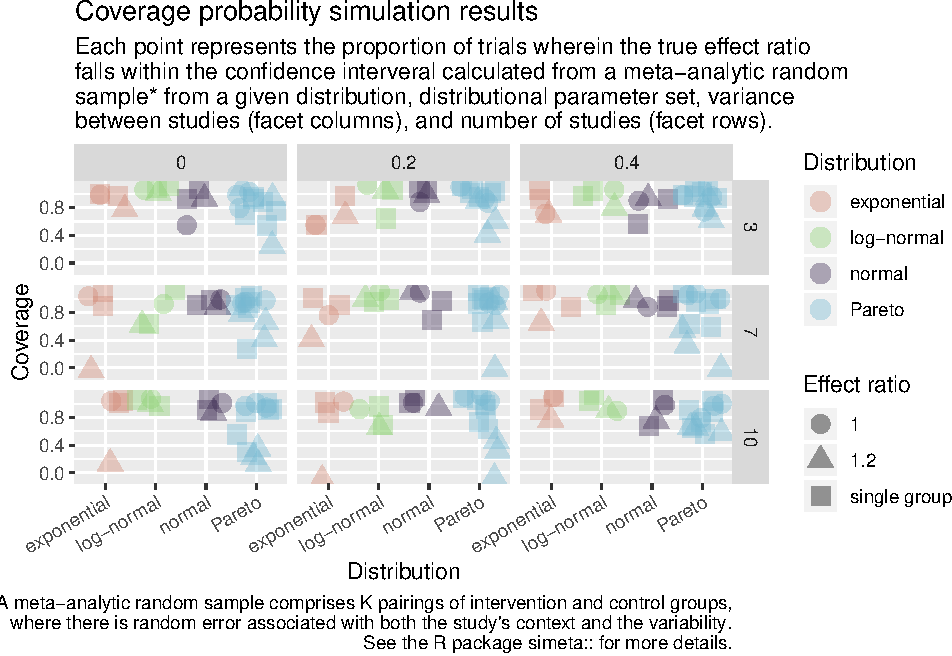
\includegraphics[width=\textwidth]{simeta-demo_files/figure-latex/coverage plot-1}

\hypertarget{components-of-simeta}{%
\section{Components of simeta}\label{components-of-simeta}}

The central motivation to modularising this package is attempting to
address how to create extendable research analyses. Perhaps not all of
the solutions provided are of use, but perhaps some components are.

In this section we describe the different classes of functions in the
\texttt{simeta::} package. These fall into roughly three categories.
Simulation-level parameters set the different parameters to simulate
over, such as number of studies or true effect ratio. Research output
tools provide outputs of the analysis for reporting, with tables and
visualisations. Finally, simulation tools, where the components of
\texttt{simeta::} have been modularised for use and extendability in
other analyses.

\hypertarget{simulation-level-parameters}{%
\subsection{Simulation-level
parameters}\label{simulation-level-parameters}}

The \texttt{metasims} function has a set of default simulation-level
parameters, \texttt{default\_parameters}. In the
\protect\hyperlink{specify-dist}{following section} it is shown how to
specify these parameters.

\begin{verbatim}
# arguments are easier to read and extract using the output of the simulation object
sims %>% 
  pluck("arguments") %>% 
    kableExtra::kable() %>% 
  kableExtra::kable_styling()
\end{verbatim}

argument

value

single\_study

FALSE

measure

median

measure\_spread

iqr

distributions

default\_parameters

k

c(3, 7, 10)

tau\_sq\_true

seq(from = 0, to = 0.4, by = 0.2)

unequal\_effect\_ratio

1.2

min\_n

20

max\_n

200

prop

0.5

prop\_error

0.1

trials

params\$trials

trial\_fn

metatrial

beep

FALSE

knha

TRUE

progress

FALSE

\begin{verbatim}
# this simulation used the same as the default arguments
\end{verbatim}

In the above table, we set simulation-level parameters: distribution
sets, \texttt{distributions}; number of studies, \texttt{k}; true
variation between the studies, \texttt{tau\_sq\_true}; unequal effect
ratio, \texttt{unequal\_effect\_ratio}, in addition to testing for no
effect; minimum, \texttt{min\_n}, and maximum, \texttt{max\_n}, expected
sample sizes with proportion, \texttt{prop}, and associated error,
\texttt{prop\_err}; and number of trials, \texttt{trials}, of each
simulation.

The distributions sampled are expected to be in the form of a table,
with one column for distributions \texttt{dist} in an R-friendly format,
and parameters \texttt{par} in a list.

\begin{verbatim}
# simeta comes with a default parameter set
default_parameters %>% 
  kableExtra::kable() %>% 
  kableExtra::kable_styling()
\end{verbatim}

dist

par

norm

list(mean = 2, sd = 0.3)

exp

list(rate = 2)

pareto

list(shape = 3, scale = 3)

pareto

list(shape = 2, scale = 1)

pareto

list(shape = 0.5, scale = 1)

lnorm

list(meanlog = 1, sdlog = 0.3)

\hypertarget{specify-dist}{%
\subsubsection{Specifying distribution parameters}\label{specify-dist}}

You can specify your

It is expected to be of the form of a \texttt{tibble} with a column,
\texttt{dist}, for R-friendly distribution names and a column,
\texttt{par}. R-friendly means by concatenating on \texttt{d},
\texttt{p}, \texttt{q}, or \texttt{r}, you obtain a distribution
function in R.

\begin{verbatim}
sims %>%
  pluck("distributions") %>% 
  sim_dist(output = "table")
\end{verbatim}

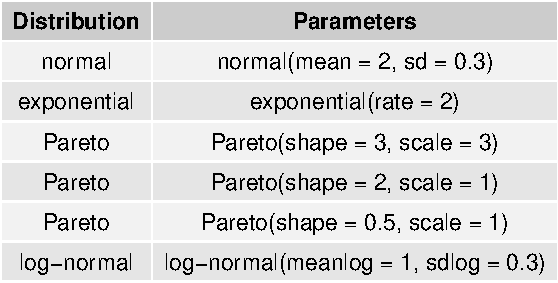
\includegraphics{simeta-demo_files/figure-latex/default parameters vis-1.pdf}

\begin{verbatim}
sims %>% 
  pluck("distributions") %>% 
  sim_dist()
\end{verbatim}

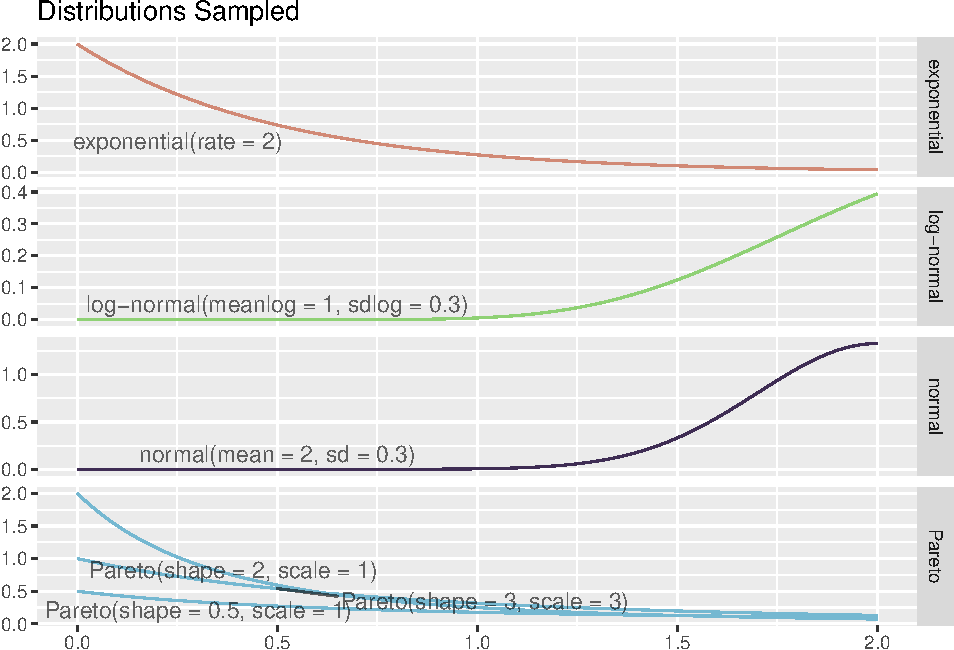
\includegraphics{simeta-demo_files/figure-latex/default parameters vis-2.pdf}

The \texttt{simeta::} package is currently coded to simulate date from
the normal, exponential, Pareto, and log-normal distributions.

The mathematical methodology to is repeated, but the derivation is
slightly different.

For these distributions, any reasonable parameter choice can be
specified via the \texttt{par} column.

\hypertarget{research-output-tools}{%
\subsection{Research output tools}\label{research-output-tools}}

Simeta provides a few research outputs, which we describe in this
section:

\begin{enumerate}
\def\labelenumi{\arabic{enumi}.}
\tightlist
\item
  Coverage plot
\item
  Distributions sampled summary tools
\item
  Simulation results as data
\end{enumerate}

\hypertarget{coverage-plot}{%
\subsubsection{Coverage plot}\label{coverage-plot}}

The coverage probability plot produced by \texttt{coverage\_plot}
summarises the proportion of trials for each metaparameter set of
distribution, variation between studies, effect ratio, and number of
studies.

\begin{verbatim}
sims %>% 
  coverage_plot()
\end{verbatim}

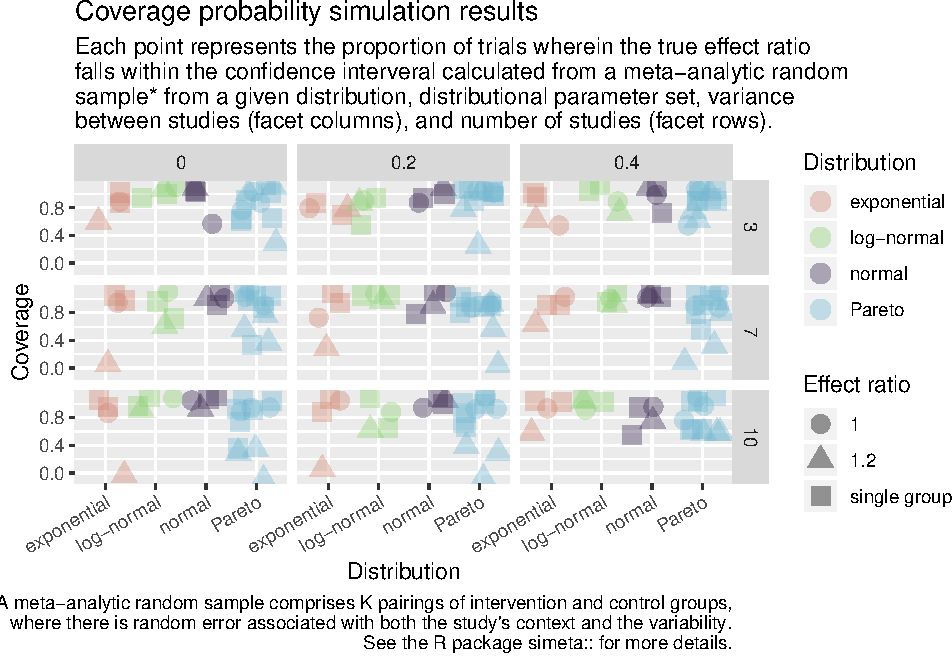
\includegraphics{simeta-demo_files/figure-latex/unnamed-chunk-2-1.pdf}

\hypertarget{distributions-summary}{%
\subsubsection{Distributions summary}\label{distributions-summary}}

There are three ways to summarise the distributions sampled in the
simulation:

\begin{enumerate}
\def\labelenumi{\arabic{enumi}.}
\tightlist
\item
  Plot
\item
  Table
\item
  R dataframe
\end{enumerate}

\begin{verbatim}
# plot
sims %>% 
  pluck("distributions") %>% 
  sim_dist()
\end{verbatim}

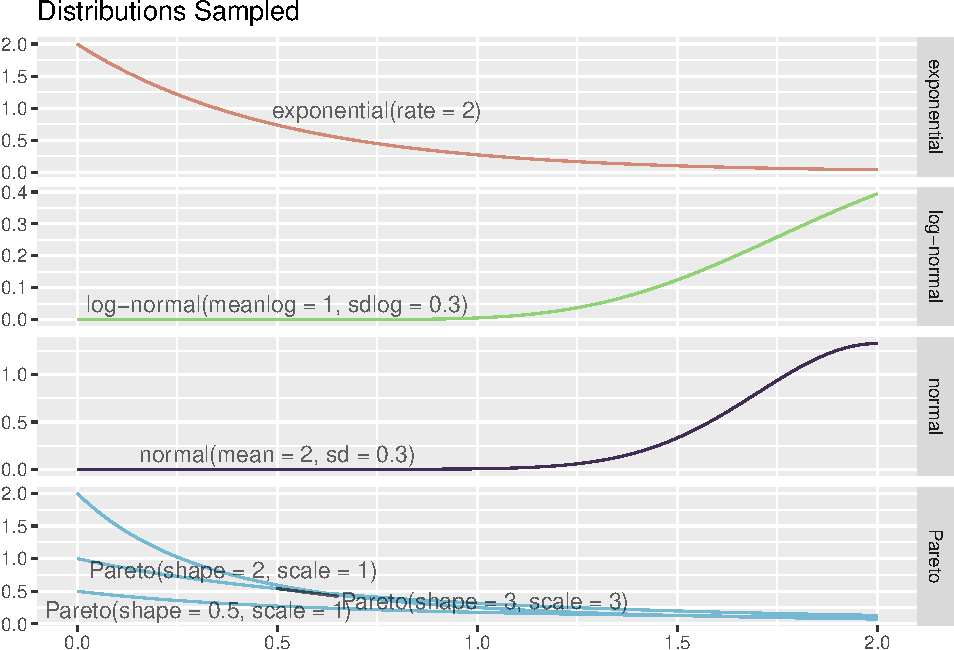
\includegraphics{simeta-demo_files/figure-latex/unnamed-chunk-3-1.pdf}

\begin{verbatim}
# table
sims %>% 
  pluck("distributions") %>% 
  sim_dist(output = "table")
\end{verbatim}

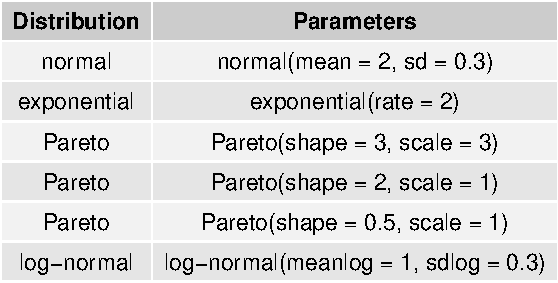
\includegraphics{simeta-demo_files/figure-latex/unnamed-chunk-3-2.pdf}

\begin{verbatim}
# data.frame
sims %>% 
  pluck("distributions")
\end{verbatim}

\begin{verbatim}
##     dist      par
## 1   norm 2.0, 0.3
## 2    exp        2
## 3 pareto     3, 3
## 4 pareto     2, 1
## 5 pareto 0.5, 1.0
## 6  lnorm 1.0, 0.3
\end{verbatim}

\hypertarget{simulation-results}{%
\subsubsection{Simulation results}\label{simulation-results}}

A list-object is returned from \texttt{metasims} that provides:

\begin{enumerate}
\def\labelenumi{\arabic{enumi}.}
\tightlist
\item
  simulation results in a tibble
\item
  simulation metaparameters in a summary tibble
\item
  simulation metaparameters, one row per simulation
\item
  simulation distributions
\end{enumerate}

\begin{verbatim}
# metasims-created object
sims %>% str(1)
\end{verbatim}

\begin{verbatim}
## List of 4
##  $ results      :Classes 'tbl_df', 'tbl' and 'data.frame':   216 obs. of  20 variables:
##  $ arguments    :Classes 'tbl_df', 'tbl' and 'data.frame':   16 obs. of  2 variables:
##  $ sim_pars     :Classes 'tbl_df', 'tbl' and 'data.frame':   108 obs. of  8 variables:
##  $ distributions:Classes 'distributions' and 'data.frame':   6 obs. of  2 variables:
##  - attr(*, "class")= chr [1:2] "sim_ma" "list"
\end{verbatim}

\begin{verbatim}
# simulation results
sims %>% pluck("results") %>% skimr::skim()
\end{verbatim}

Data summary

Name

Piped data

Number of rows

216

Number of columns

20

\_\_\_\_\_\_\_\_\_\_\_\_\_\_\_\_\_\_\_\_\_\_\_

Column type frequency:

character

4

list

3

numeric

13

\_\_\_\_\_\_\_\_\_\_\_\_\_\_\_\_\_\_\_\_\_\_\_\_

Group variables

None

\textbf{Variable type: character}

skim\_variable

n\_missing

complete\_rate

min

max

empty

n\_unique

whitespace

measure

0

1.0

6

9

0

2

0

id

0

1.0

5

7

0

108

0

effect\_ratio

108

0.5

8

8

0

2

0

rdist

0

1.0

3

6

0

4

0

\textbf{Variable type: list}

skim\_variable

n\_missing

complete\_rate

n\_unique

min\_length

max\_length

parameters

0

1

6

1

2

n

0

1

108

3

3

sim\_results

0

1

108

12

12

\textbf{Variable type: numeric}

skim\_variable

n\_missing

complete\_rate

mean

sd

p0

p25

p50

p75

p100

hist

tau\_sq

0

1

0.10

0.18

0.00

0.00

0.03

0.13

1.34

▇▁▁▁▁

ci\_width

0

1

0.88

1.00

0.05

0.29

0.61

1.03

7.13

▇▁▁▁▁

bias

0

1

-0.10

0.22

-1.01

-0.17

-0.02

0.02

0.31

▁▁▂▇▂

coverage\_count

0

1

2.59

0.73

0.00

2.00

3.00

3.00

3.00

▁▁▁▂▇

successful\_trials

0

1

3.00

0.00

3.00

3.00

3.00

3.00

3.00

▁▁▇▁▁

coverage

0

1

0.86

0.24

0.00

0.67

1.00

1.00

1.00

▁▁▁▂▇

errors

0

1

0.00

0.00

0.00

0.00

0.00

0.00

0.00

▁▁▇▁▁

warnings

0

1

0.00

0.00

0.00

0.00

0.00

0.00

0.00

▁▁▇▁▁

messages

0

1

3.00

0.00

3.00

3.00

3.00

3.00

3.00

▁▁▇▁▁

result

0

1

3.00

0.00

3.00

3.00

3.00

3.00

3.00

▁▁▇▁▁

k

0

1

6.67

2.87

3.00

3.00

7.00

10.00

10.00

▇▁▇▁▇

tau\_sq\_true

0

1

0.20

0.16

0.00

0.00

0.20

0.40

0.40

▇▁▇▁▇

true\_effect

0

1

1.54

1.08

0.35

0.41

1.39

2.72

3.00

▇▁▁▂▅

\begin{verbatim}
# simulation metaparameters summary
sims %>% pluck("arguments") %>% 
  kableExtra::kable() %>% kableExtra::kable_styling()
\end{verbatim}

argument

value

single\_study

FALSE

measure

median

measure\_spread

iqr

distributions

default\_parameters

k

c(3, 7, 10)

tau\_sq\_true

seq(from = 0, to = 0.4, by = 0.2)

unequal\_effect\_ratio

1.2

min\_n

20

max\_n

200

prop

0.5

prop\_error

0.1

trials

params\$trials

trial\_fn

metatrial

beep

FALSE

knha

TRUE

progress

FALSE

\begin{verbatim}
# simulation metaparameters, one row per simulation
sims %>% pluck("sim_pars") %>% head() %>% select(1:5) %>% 
  kableExtra::kable() %>% kableExtra::kable_styling()
\end{verbatim}

k

tau\_sq\_true

effect\_ratio

rdist

parameters

3

0

1

norm

list(mean = 2, sd = 0.3)

3

0

1

exp

list(rate = 2)

3

0

1

pareto

list(shape = 3, scale = 3)

3

0

1

pareto

list(shape = 2, scale = 1)

3

0

1

pareto

list(shape = 0.5, scale = 1)

3

0

1

lnorm

list(meanlog = 1, sdlog = 0.3)

\begin{verbatim}
# simulation distributions summary
sims %>% pluck("distributions") %>% 
  kableExtra::kable() %>% kableExtra::kable_styling()
\end{verbatim}

dist

par

norm

list(mean = 2, sd = 0.3)

exp

list(rate = 2)

pareto

list(shape = 3, scale = 3)

pareto

list(shape = 2, scale = 1)

pareto

list(shape = 0.5, scale = 1)

lnorm

list(meanlog = 1, sdlog = 0.3)

\hypertarget{simulation-tools}{%
\subsection{Simulation tools}\label{simulation-tools}}

The components of \texttt{simeta::} are deliberately modularised, with
the intention of facilitating future optimisation and improvements.

\end{document}
